%%%%%%
% $Beschreibung: Aufbau eines Schrittmotors $
% $Autor: ter Veen $
% $Datum: 22.06.2024 $
% $Version: 1 $
% $Pfad: SchrittmotorArduino/DevoloperDoc/tikz/AufbauSchrittmotor.tex $
%
%%%%%%

	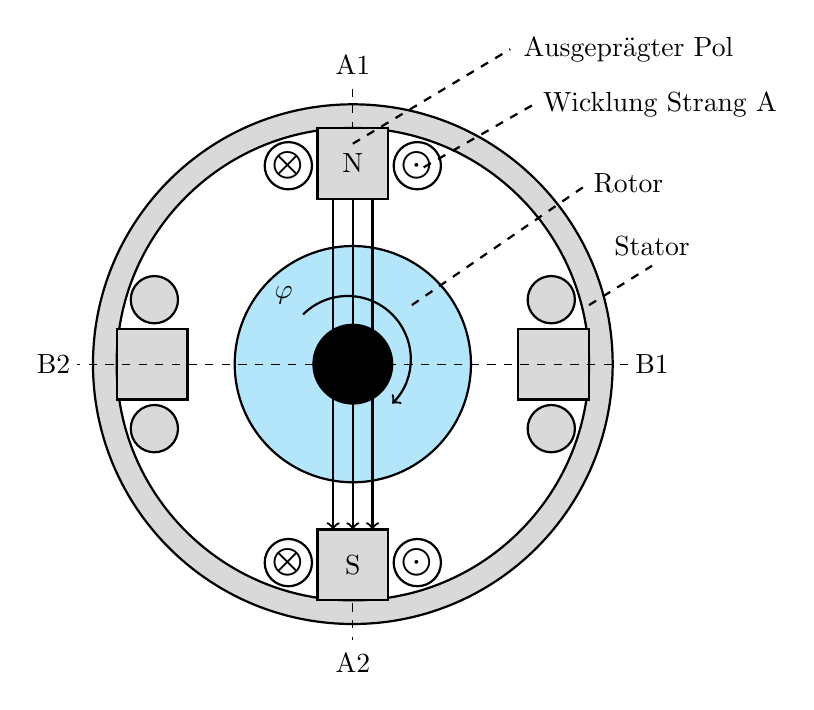
\begin{tikzpicture}
		% stator
		\draw[thick,fill=gray!30] (0,0) circle (3.3);
		\draw[thick, fill=white] (0,0) circle (3);
		
		% Achse
		\draw[dashed] (0,3.5) -- (0,-3.5);
		
		% Polung
		\draw[thick,fill=gray!30] (-0.45,3) rectangle (0.45,2.1) node[midway] {N};
		\draw[thick,fill=gray!30] (-0.45,-3) rectangle (0.45,-2.1) node[midway] {S};
		
		\draw[thick,fill=gray!30] (3,-0.45) rectangle (2.1,0.45) node[midway] {};
		\draw[thick,fill=gray!30] (-3,-0.45) rectangle (-2.1,0.45) node[midway] {};
		
		% rotor
		\filldraw[fill=cyan!30, thick] (0,0) circle (1.5);
		\filldraw[fill=black, thick] (0,0) circle (0.5);
		
		% Spulen
		\foreach \angle in {108, -108} {
			\draw[thick] (\angle:2.65) circle (0.3);
			\node at (\angle:2.65) {\small $\bigotimes$};
		}
		
		\foreach \angle in {72, -72} {
			\draw[thick] (\angle:2.65) circle (0.3);
			\node at (\angle:2.65) {\small $\bigodot$};
		}
		
		\foreach \angle in {18, -18, 162, -162} {
			\draw[thick, fill=gray!30] (\angle:2.65) circle (0.3);
			\node at (\angle:2.65) {};
		}
		
		% labels
		\node at (0,3.8) {A1};
		\node at (0,-3.8) {A2};
		\node at (3.8,0) {B1};
		\node at (-3.8,0) {B2};
		
		\node[align=center] at (3.5,4) {Ausgeprägter Pol};
		\draw[dashed,thick] (0,2.8) -- (2,4);
		
		\node[align=center] at (3.9,3.3) {Wicklung Strang A};
		\draw[dashed,thick] (0.9,2.5) -- (2.3,3.3);
				
		\node[align=center] at (3.5,2.3) {Rotor};
		\draw[dashed,thick] (0.75,0.75) -- (3,2.3);
		
		\node[align=center] at (3.8,1.5) {Stator};
		\draw[dashed,thick] (3,0.75) -- (3.8,1.25);
		
		% Magnetfeld
		\draw[->, thick] (0.25,2.1) -- (0.25,-2.1);
		\draw[->, thick] (0,2.1) -- (0,-2.1);
		\draw[->, thick] (-0.25,2.1) -- (-0.25,-2.1);
		
		% Achse
		\draw[dashed] (3.5,0) -- (-3.5,0);
		
		 % phi
		\draw[<-, thick] (0.5,-0.5) arc[start angle=-45, end angle=135, radius=0.8] node[above left] {$\varphi$};
		
	\end{tikzpicture}
